% Drawing 154/08-30 -- folder 154, batch 08, archive page 156 (PDF page 157).
% Transcription: après $(D_0, \beta^{*}, -\omega^{*})$, un petit dessin en couleur : deux droites orange qui se croisent ; une droite verte en tirets passe par le croisement, une droite verte pleine passe au-dessous (le triangle entre les deux hachuré au crayon) ; à droite, une flèche verte transverse vers le haut et une flèche verte vers la gauche marquée $-\omega^{*}$
% Kind: orange crossing with dashed green line through it, solid green line below, hatched triangle; arrows up and left, -omega*. Method 2 (schematic redraw from the facsimile). Status: ok.
% Notes: Small drawing after the triple (D_0, beta*, -omega*). Two orange lines crossing (the right-hand stroke is bowed on the page; it is drawn as two straight halves meeting at the crossing); a dashed green line through the crossing; a solid green line below, the triangle between it and the crossing hatched in pencil; to the right a transverse green arrow pointing up across the dashes, and below the dashes a green arrow pointing left with « -omega* » in pencil under it. 2 orange strokes, 1 crossing, 6 dashes, 2 arrows, 1 label. Read from the 400 dpi colour scan; each pair of orange strokes fitted to the ink and drawn through its computed crossing, the triangles bounded by the computed intersections with the green line; the redraw was overlaid on the scan and agrees to within a stroke's width. The felt strokes are drawn straight (slight curvature of a few strokes not reproduced). Redrawn 2026-11-12 (issue 128): to check again.
% Coordinates: 1 unit = 1 mm = 1/100 of the crop width, same scale on both axes (bbox in page fractions: [0.661, 0.247, 0.765, 0.298]).
% Redrawn by Claude (claude-fable-5-2), issue #128, 2026-11-12; not checked by a human; not compiled (no TeX in the session).
% Rights: reproduces part of the work -- behind RENDER_TRANSCRIPTS, never published by itself.
\documentclass[tikz,border=3pt]{standalone}
\usepackage{amsmath,amssymb}
\usetikzlibrary{patterns,arrows.meta}
\tikzset{Or/.style={orange!90!black}, Lg/.style={green!60!black!70}, Br/.style={brown!80!black}, pencil/.style={black!55}, mpt/.style={circle,draw,inner sep=1.3pt}, pt/.style={circle,fill,inner sep=0.9pt}}
\colorlet{Or}{orange!90!black}\colorlet{Lg}{green!60!black!70}\colorlet{Br}{brown!80!black}
\begin{document}
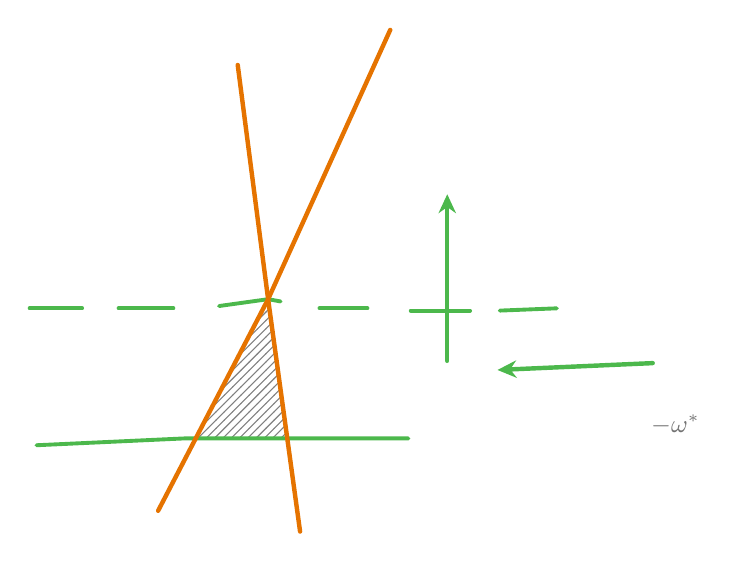
\begin{tikzpicture}[x=1mm,y=1mm,line cap=round,line join=round,font=\scriptsize]
\path[pattern=north east lines,pattern color=black!50] (33.19,-37.1) -- (23.99,-54.78) -- (35.62,-54.78) -- cycle;
\draw[Lg,line width=1.4pt] (3.77,-55.65) -- (22.61,-54.78) -- (51.01,-54.78);
\draw[Lg,line width=1.4pt] (2.9,-38.26) -- (9.57,-38.26);
\draw[Lg,line width=1.4pt] (14.2,-38.26) -- (21.16,-38.26);
\draw[Lg,line width=1.4pt] (26.96,-37.97) -- (33.19,-37.1) -- (34.78,-37.39);
\draw[Lg,line width=1.4pt] (39.71,-38.26) -- (45.8,-38.26);
\draw[Lg,line width=1.4pt] (51.3,-38.55) -- (58.84,-38.55);
\draw[Lg,line width=1.4pt] (62.61,-38.55) -- (69.86,-38.26);
\draw[Or,line width=1.6pt] (48.7,-2.9) -- (33.19,-37.1) -- (19.22,-63.97);
\draw[Or,line width=1.6pt] (29.33,-7.36) -- (33.19,-37.1) -- (37.25,-66.61);
\draw[Lg,line width=1.6pt,-{Stealth[length=2.4mm,width=2.2mm]}] (55.94,-44.93) -- (55.94,-23.77);
\draw[Lg,line width=1.6pt,-{Stealth[length=2.4mm,width=2.2mm]}] (82.03,-45.22) -- (62.32,-46.09);
\node[pencil,inner sep=1pt] at (84.93,-53.04) {\small $-\omega^{*}$};
\end{tikzpicture}
\end{document}
